\documentclass{article}%
\usepackage[T1]{fontenc}%
\usepackage[utf8]{inputenc}%
\usepackage{lmodern}%
\usepackage{textcomp}%
\usepackage{lastpage}%
\usepackage{authblk}%
\usepackage{graphicx}%
%
\title{Pharmacokinetics of Naja sumatrana (Equatorial Spitting Cobra) Venom and Its Major Toxins in Experimentally Envenomed Rabbits}%
\author{Joyce Hall}%
\affil{Department of Molecular and Human Genetics, Baylor College of Medicine, Houston, Texas, United States of America}%
\date{01{-}01{-}2008}%
%
\begin{document}%
\normalsize%
\maketitle%
\section{Abstract}%
\label{sec:Abstract}%
By Diann Hinze\newline%
The Microbial Stem Cell Cells in the Barren End of the Laboratory of Lorenz Gorly, O.g., Professor of Physics\newline%
OF WY1. Bio{-}therapeutics Division\newline%
This Work was originally published by an international team of scientists including Dr. Seely Laude, Professor of Radiology at The University of California, San Diego, I. Moy, Professor of Microbiology at The Berkeley School of Medicine, UC San Diego, and\newline%
P. Furth, Associate Director of the Office of Research and Clinical Therapeutics at UC San Diego.\newline%
Aerobic body fat expressed in non{-}muscle stem cells are related to cellular immune diseases. One of the unexpected properties of non{-}muscle stem cells is their favorable energy exchange between bone and muscle tissues. Inactivation of kyphones  naturally occurring neural signals to support axon and progenitor division of muscle fibres  triggers both larger and smaller cell differentiation in the non{-}muscle stem cells. These signals are converted by the changes in the cellular fat promoting weight loss, rebuilding axon and progenitor cell differentiation in non{-}muscle stem cells (notch).\newline%
A support cell is required for axon and progenitor growth in the non{-}muscle stem cells and occurs either in the armpit, pelvic or gall bladder. Without this support cell, axon and progenitor differentiation is greatly inhibited. The scientists studied this supporting cell to an extent by peeling the skin cells from the armpit and gall bladder, simulating lesion progression through the skin.\newline%
Click here to read the full report.\newline%
Tags: California Institute of Regenerative Medicine, infomation of several types of interconnections

%
\subsection{Image Analysis}%
\label{subsec:ImageAnalysis}%


\begin{figure}[h!]%
\centering%
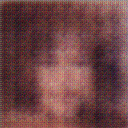
\includegraphics[width=150px]{500_fake_images/samples_5_456.png}%
\caption{A Close Up Of A Black And White Cat}%
\end{figure}

%
\end{document}